\chapter{Программный комплекс и численные примеры решения задач представленных математических моделей}\label{part4}

В данной главе представлены описание и структура программно-вычислительного комплекса, предназначенного для расчета задачи оптимального размещения БС.

\section{Программный комплекс расчета задачи размещения БС}

Программный комплекс представляет собой реализацию на языке Python алгоритма типа ветвей и границ комбинаторной задачи оптимизации поиска максимального телекоммуникационного покрытия при размещении базовых станций. Код программы представлен в \url{https://github.com/m0000Amir/BST_BS_types_set}.

Структура программно-вычислительного комплекса представлена на рисунке \ref{fig:part4_program_computer}. На вход подается JSON-file, содержащий параметры конфигурации и входные данные задачи.

 Параметы конфигурации расположены под ключом $\textbf{configuration}$ (Рисунок \cref{fig:part4_input_data_configuration}):
 \begin{itemize}
   \item $\textbf{method}$ -- метод решения задачи размещения. Значение $\textit{bab}$ -- метод ветвей и границ или $\textit{bf}$  -- метод полного перебора;
   \item $\textbf{estimation\_method}$ -- метод расчета оценки недопокрытия справа. Значение $\textit{LP}$ -- решение с помощью сиплекс-метода, значение $\textit{ILP}$ -- решение с помощью задача целочисленного линейного программирования или значение $\textit{knapsack}$ -- решение с помощью задачи <<О ранце>>;
   \item $\textbf{placed\_all\_station}$ -- частный случай задачи размещения, когда отсутствуют ограничения на стоимость и времени задержки, в такой постановке размещается все множество БС. Принимает значения $\textit{True}$ или $\textit{False}$;
   \item $\textbf{drawing}$ -- отрисовка полученного дерева решения.  Принимает значения $\textit{True}$ или $\textit{False}$;
   \item $\textbf{last\_optimal\_noncoverage}$ -- полученное оптимальное недопокрытия на последнем решении  для задачи поиска последовательности лучших решений. Принимает любые положительные действительные значения;
   \item $\textbf{relation\_deviation}$ -- заданное отклонение в процентах от полученного оптимального решения для задачи поиска последовательности лучших решений.
 \end{itemize}



\begin{figure}[h!]
  \centering
   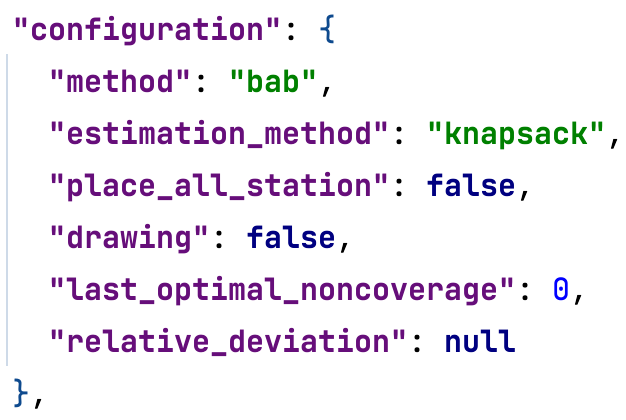
\includegraphics[width=.5\textwidth]{input_data_configuration.png}
\caption{Параметры конфигурации}
\label{fig:part4_input_data_configuration}
\end{figure}

Файл JSON содержит входные данные задачи оптимизации: 
\begin{itemize}
  \item координаты размещения $\textbf{placement}$ и координаты размещения шлюзов $\textbf{gateway\_placement}$;
  \item  параметры антенн шлюзов $\textbf{gateway}$ и абонентских устройств $\textbf{user\_device}$;
  \item ограничения задачи на стоимость $\textbf{cost\_limit}$ и время задержки $\textbf{delay\_limit}$;
  \item параметры для расчета дальности телекоммуникационного покрытия: несущая частота $\textbf{frequency}$, запас на замирания сигнала $\textbf{link\_som}$ и $\textbf{coverage\_som}$;
  \item параметры для расчета задержек: средний размер пакетов $\textbf{average\_packet\_size}$ и интенсивность входящего потока $\textbf{arrival\_rate}$;
  \item $\textbf{sta}$ -- множество заданных БС.
\end{itemize}

\begin{figure}[h!]
  \centering
   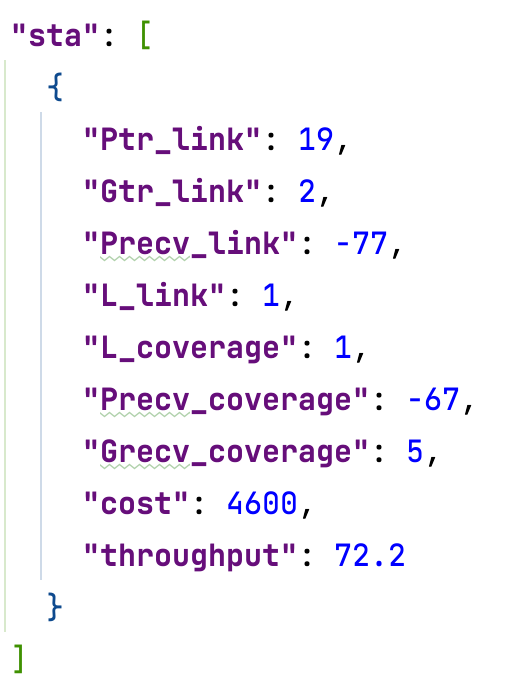
\includegraphics[width=.4\textwidth]{input_data_sta.png}
\caption{Параметры БС}
\label{fig:part4_input_data_sta}
\end{figure}

Каждый элемент массива $\textbf{sta}$ (Рисунок \cref{fig:part4_input_data_sta}) представляет собой JSON-объект и содержит следующие параметры:
\begin{itemize}
  \item $\textbf{Ptr\_link}$ -- мощность антенны, обеспечивающей телекоммуникационную связь между станциями;
  \item $\textbf{Gtr\_link}$ -- усиления антенны, обеспечивающей телекоммуникационную связь между станциями;
  \item $\textbf{Precv\_link}$ -- чувствительность антенны, обеспечивающей телекоммуникационную связь между станциями;
  \item $\textbf{L\_link}$ -- потери сигнала в кабеле и разъемах передающего тракта антенны, обеспечивающей телекоммуникационную связь между БС;
  \item $\textbf{L\_coverage}$ -- потери сигнала в кабеле и разъемах передающего тракта антенны, обеспечивающей телекоммуникационное покрытие БС;
  \item $\textbf{Precv\_coverage}$ -- чувствительность антенны, обеспечивающей телекоммуникационное покрытие БС;
  \item $\textbf{Grecv\_coverage}$ -- усиления антенны, обеспечивающей телекоммуникационное покрытие БС;
  \item $\textbf{cost}$ -- стоимость БС;
  \item $\textbf{throughput}$ -- пропускная способность БС.
\end{itemize}



\begin{figure}[h!]
  \centering
   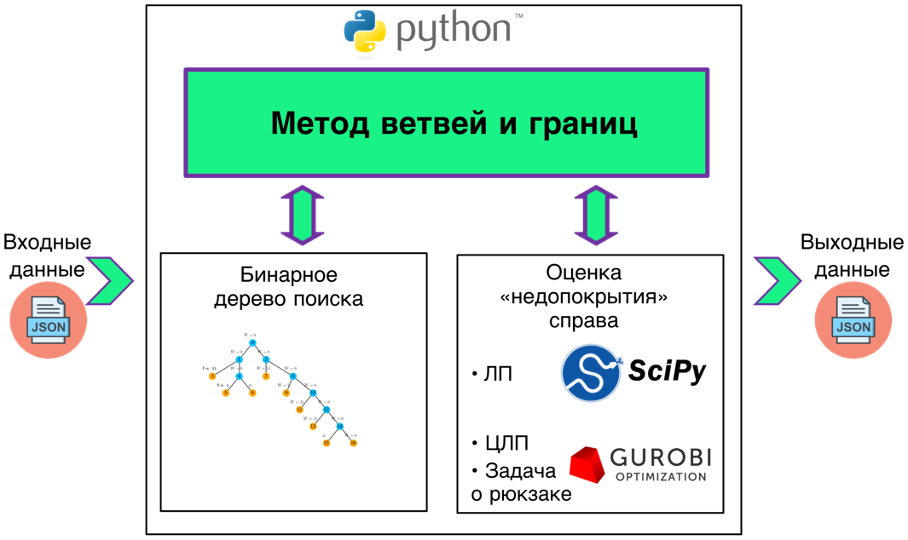
\includegraphics[width=.95\textwidth]{program_computer.png}
\caption{Cтруктура программно-вычислительного комплекса}
\label{fig:part4_program_computer}
\end{figure}

Перед тем как приступить к задаче размещения, необходимо подготовить параметры для каждой БС: радиус связи между станциями и радиус покрытия БС. Параметры рассчитываются в блоке расчета дальности телекоммуникационной связи с помощью уравнения энергетического потенциала линии связи и модели распространения сигнала. Модели распространения представлены в главе 1.


Задача размещения БС представлена в виде комбинаторной модели в экстремальной форме. Алгоритм поиска оптимального размещения относится к типу ветвей и границ. 

Для поиска оптимального размещения используется процедура построения бинарного дерева поиска. На каждом шаге проверяется условия на возможность закрытие узла дерева. Построение бинарного дерева поиска реализовано рекуррентным способом.

Блок расчета оценки недопокрытия справа представляет собой решение задачи оптимизации. Блок содержит три варианта расчета оценки. \underline{\textit{\textbf{Задача 2}}} представляет собой задачу ЦЛП, \underline{\textit{\textbf{задача 3}}} является задачей <<О ранце>>. \underline{\textit{\textbf{Задача 4}}} представляет собой задачу ЛП. Задача ЦЛП и задача <<О ранце>> рассчитывается в коммерческом продукте расчета задач дискретной оптимизации Gurobi Optimizer \cite{gurobi}. Задача ЛП решается с использованием библиотеки для языка программирования Python с открытым исходным кодом SciPy \cite{scipy}. 


\begin{figure}[h!]
  \centering
   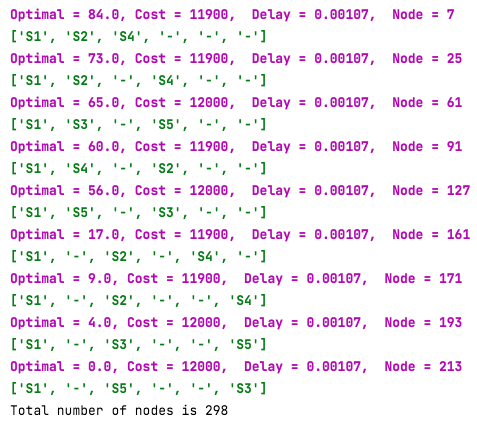
\includegraphics[width=.6\textwidth]{problem_output.png}
\caption{Пример полученного решения задачи}
\label{fig:part4_problem_output}
\end{figure}

В ходе движения по дереву поиска записываются все полученные рекорды \textbf{Optimal} (Рисунок \cref{fig:part4_problem_output}). Также записываются стоимость размещения \textbf{Cost}, время межконцевой задержки \textbf{Delay} и номер узла дерева \textbf{Node}, на котором был получен рекорд. Для каждого рекорда записывается множество размещенных БС. Последний полученный рекорд является оптимальным решением задачи. Решение задачи записывается в выходной JSON-файл.

% Алгоритм на основе метода ветвей и границ основан на следующих построениях, позволяющих уменьшить время перебора:


% \begin{enumerate}
%   \item Ветвление. Разбиение исходного множества на попарно не пересекающие дочерние подмножества в ходе поиска оптимального решения.
%   \item Получение нижних границ. Исследования текущей вершины на возможность закрытия.
% \end{enumerate}

% Особенность задачи дискретного программирования состоит в том, что они имеют переборный характер. Основная идея комбинаторных алгоритмов -- выделить из множества допустимых решений подмножества, не содержащие оптимальных решений \cite{SigalBook}, для сокращения времени перебора всех возможных вариантов. 


% Опишем процедуру построения бинарного дерева поиска (дерева ветвлений) для полного перебора без повторений всех элементов множества $\Gamma$. Данная процедура будет использована при построении дерева поиска в алгоритме МВиГ решения \textbf{задачи 1}.

% Предполагается, что в множестве $S$ станции упорядочены по не убыванию радиусов покрытия. Описываемая процедура использует известный прием разбиения множества $G$ на подмножества с использованием некоторого параметра. Процесс формирования и последовательность исследования подмножеств обычно представляется с помощью дерева поиска, представляющего собой ориентированное от корня «дерева ветвлений», где каждому подмножеству соответствует вершина на дереве. Множеству $\Gamma$ соответствует корневая вершина. 


\section{Численный пример оптимального размещения базовых станций сети с линейной топологией в виде задачи целочисленного линейного программирования}\label{part4:ilp_solution}

\fixme{Переделать численный пример}
В этой секции представлен численный пример решения данной задачи.
% This section shows one simple case of the problem.

Задан линейный участок $L$ с длиной 300 с количеством $n=7$ точек размещения. Координаты точек размещения представлены в таблице \cref{tab:part3_placed_point}.  Задан бюджет размещения $C=130$. Центральная частота $f = 2437$ МГц. 

\begin{table}[h!]\centering
  \begin{tabular}{|c||c|c|c|c|c|c|c|}\hline
    $a_i$ & $a_1$ &  $a_2$ & $a_3$ & $a_4$ & $a_5$ & $a_6$ & $a_7$ \\ \hline \hline
    Координата & 29 & 40 & 95 & 139 & 181 & 230 & 273 \\ \hline
\end{tabular}\caption{Точки размещения участка с длиной $L = 300$.}\label{tab:part3_placed_point}
\end{table}

Задано множества БС $m = 8$ с параметрами представленными в таблице \cref{tab:part3_BS}. Также в таблице представлены параметры шлюзов и контролируемых объектов. Параметры объектов необходимы для расчета радиусов покрытия станций.

\begin{table}[b]\centering
  \begin{tabular}{|c||c|c|c|c|c|c|c|}\hline
    BS & $P_{tr}^R$ &  $G_{tr}^R$ & $P_{recv}^R$ & $P_{recv}^r$ & $G_{recv}^r$ & $c$ \\ \cline{2-1} \cline{3-1} \cline{4-1} \cline{5-1}  \cline{6-1} \cline{7-1}
     & дБм & дБ & Дбм & дБм & дБ & у.е.  \\ \hline
    1 & 20 & 5 & -69 & -67 & 5 & 40 \\ 

    2 & 19 & 5 & -67 & -67 & 5 & 28 \\ 

    3 & 18 & 5 & -69 & -67 & 5 & 45 \\ 

    4 & 19 & 5 & -69 & -67 & 6 & 22 \\ 

    5 & 19 & 5 & -67 & -67 & 5 & 21 \\ 

    6 & 20 & 5 & -69 & -67 & 5 & 40 \\ 

    7 & 19 & 5 & -67 & -67 & 5 & 28 \\

    8 & 18 & 5 & -69 & -67 & 5 & 45 \\ \hline \hline  

    &  $G_{recv}^R$ & $P_{recv}^R$ &  & & $P_{tr}^r$ & $G_{tr}^r$ \\  \cline{2-1} \cline{3-1} \cline{6-1} \cline{7-1} 

    Шлюз& дБ & дБм & & Объект & дБм & дБ  \\  \cline{2-1} \cline{3-1}  \cline{6-1} \cline{7-1}

    &  5 & -69 & &  & 15 & 2  \\ \hline

  \end{tabular}\caption{Параметры станций, шлюзов и объектов.}\label{tab:part3_BS} 
\end{table}

\textbf{Расчет радиуса связи между станциями}
Все БС оснащены направленной антенной с высоким коэффициентом усиления для связи с соседними станциями.
Для расчета потерь между станциями $j$ и $q$ воспользуемся формулой (\ref{eq:part3_L_fs_from_link_budget}):

\begin{displaymath}
  L_{fs}^{jq} = P_{tr}^R(j) - L_{tr} + G_{tr}^R(j) + G_{tr}^R(q) - L_{recv} - SOM - P_{recv}^R(q).
\end{displaymath}


Потери на кабелях приемнике $ L_{recv} $ и передатчике $ L_{tr} $ примем равным 1 дБ и запас на замирания сигнала $ SOM = 10 $ дБ.

% Let us carry out an example of the calculation communication link between stations $ s_1 $ and $ s_2 $:
Для примера рассчитаем радиус связи между станциями $ s_1 $ и $ s_2 $:

\begin{align}
  \begin{aligned}
  L_{fs}^{12} = P_{tr}^R(1) - L_{tr} + G_{tr}^R(1) + G_{tr}^R(2) - L_{recv} - SOM - P_{recv}^R(2)= \\
  = 20 - 1 + 5 + 5 - 1 - 10 - (-69) = 87 (dB).
  \end{aligned}
\end{align}

Для расчета канала связи необходимо использовать формулу \cref{eq:part1_fspl_model_r}. Несущая частота $ f = 2437 $ МГц и коэффициент для расчета потерь $ K = -27,55 $:

\fixme{Формула не верна расчета $R_{jq}$}

\begin{align}
  \begin{aligned}
  R_{jq} = 10^{\left(\frac{L_{fs}^{jq} - 20\lg{F} - K}{20}\right)}
  = 10^{\left(\frac{87 - 20\lg{2437} - (-27.55)}{20}\right)} = 174 (m).
  \end{aligned}
\end{align}

В таблице \cref{tab:part3_Rjq} приведены расчеты максимальных радиусов связи между всеми станциями $ s_j $, $ j = 1, ..., m $ и шлюзом $ s_ {m + 1} $.

\begin{table}[h!]\centering
  \begin{tabular}{|c||c|c|c|c|c|c|c|c|c|}\hline
      $R_{jq}$ & $s_1$ & $s_2$ & $s_3$ & $s_4$ & $s_5$ & $s_6$ & $s_7$ & $s_8$ & $s_{m+1}$ \\ \hline \hline

      $s_1$ &--& 174& 219& 219& 174& 219& 174& 219& 219\\ 
      $s_2$ &195& --& 195& 195& 155& 195& 155& 195& 195\\ 
      $s_3$ &174& 138& --& 174& 138& 174& 138& 174& 174\\ 
      $s_4$ &195& 155& 195& --& 155& 195& 155& 195& 195\\ 
      $s_5$ &195& 155& 195& 195& --& 195& 155& 195& 195\\ 
      $s_6$ &219& 174& 219& 219& 174& --& 174& 219& 219\\
      $s_7$ &195& 155& 195& 195& 155& 195& --& 195& 195\\ 
      $s_8$ &174& 138& 174& 174& 138& 174& 138& --& 174\\ 
      \hline

\end{tabular}\caption{Рассчитанные радиусы связи между станциями}\label{tab:part3_Rjq}
\end{table}

\textbf{Расчет радиуса покрытия}

% Для покрытия заданного участка базовая станция оснащена всенаправленной антенной с выходной мощностью $ P_{tr}^r $ и усилением $ G_{tr}^r$. Потери в кабеле $ L_ {tr} $ равно 1.

% To cover a given section, the base station is equipped with an isotropic antenna with output power $ P_ {tr} ^ r $ and gain $ G_ {tr} ^ r $ is equal to 0. The cable loss $ L_ {tr} $ is equal to 1.

% A coverage area depends on a base station, as well as user device characteristics. Let us consider a user device with an antenna sensitivity $P_{RX} = -67$ dBm and gain $G_{RX} = 0$. Loss $L_{RX}$ is equal to 0.
Расчет проводится аналогично расчета радиусу связи между станциями. 
Потери в свободном пространстве для канала между $j$-ой БС и контролируемым объектом

\begin{displaymath}
  L_{fs}^{j} = P_{tr}^r(j) - L_{tr}  - SOM - P_{RX}. 
\end{displaymath}


Пример расчечта радиуса покрытия для  $1$-ой БС:

\begin{align}
    \begin{aligned}
  L_{fs}^{1} = P_{tr}^r + G_{tr}^r + G_{recv}^r(1) - L_{recv}(1)  - SOM - P_{recv}^r(1) = \\
 = 15+2+5-1-(-67)-10 = 78 \text{ (дБ)}.
    \end{aligned}
\end{align}

\begin{displaymath}
  r_{1} = 10^{\left(\frac{78 - 20\lg{2437} - (-27.55)}{20}\right)} = 77 \text{ (м)}.
\end{displaymath}

Рассчитанные радиусы покрытия для всех БС $ s_j $, $ j = \overline{1, m} $ представлены в таблице \cref{tab:part3_rj}).

\begin{table}[h!]\begin{center}
  \begin{tabular}{|c||c|c|c|c|c|c|c|c|}\hline
      STA & $s_1$ & $s_2$ & $s_3$ & $s_4$ & $s_5$ & $s_6$ & $s_7$ & $s_8$\\ \hline \hline

      $r_{j}$ & 77 & 77 & 77 & 87 & 77 & 77 & 77 & 77\\ \hline

\end{tabular}\caption{Рассчитанные радиусы покрытия станций}\label{tab:part3_rj}
\end{center}\end{table}

Задача ЦЛП решена с помощью Optimization Toolbox MatLab. Таблица \cref{tab:part3_ilp_solution} содержит все полученные целочисленные решения.


\begin{table}[h!]\tiny\centering
  \begin{tabular}{|c||c|c|c|c|c|c|c||c|c|}\hline
    $a_i$ & $a_1$ &  $a_2$ & $a_3$ & $a_4$ & $a_5$ & $a_6$ & $a_7$  & Покрытие & Цена \\ \hline 
    Координаты & 29 & 40 & 95 & 139 & 181 & 230 & 273 & м & у.е.\\ \hline \hline
    Целлочисленное решение 1 & $s_1$ & $s_2$ & $s_6$ & -- & -- & -- & $s_4$ & 286 & 130\\ 
    Целлочисленное решение 2 & $s_4$ & -- & $s_5$ & $s_7$ & -- & -- & $s_2$ & 289 & 99\\
    Оптимальное решение & $s_4$ & $s_2$ & -- & -- & $s_1$ & -- & $s_5$ & 300 & 111 \\ \hline
\end{tabular}\caption{Решение задачи ЦЛП.}\label{tab:part3_ilp_solution}
\end{table}

\fixme{=================================================}
\section{Численный пример оптимального размещения базовых станций сети с линейной топологией в виде экстремальной задачи в комбинаторной форме}\label{part4:bnb_solution}



Дано:
\begin{itemize}
  \item линейный участок $L =300$ метров;
  \item множество точек размещения $|A| =8$;
  \item множество БС $|S| =8$;
  \item протокол IEEE 802.11n;
  \item ограничение на суммарную стоимость $T =0.001$с;
  \item интенсивность входящих пакетов $\lambda = 1000$ 1/c;
  \item средний размер входящих пакетов $w = 1500$ байт;
  \item отклонение от оптимального решения, $\varepsilon=0.5$%
\end{itemize}

Рассмотрим пример задачи оптимального размещения БС вдоль линейного участка для организации БШС. В данном приложении будет представлен пример решения на базе семейства протоколов IEEE 802.11. Задан линейный участок $L =230$ метров. На данном участке задано множество точек размещения  $|A| =6$ с координатами, представленными в таблице \cref{tab:placement_point}. Задано множество БС $|S| =5$, таблице \cref{tab:sta_parameters}. 


% $\{36, 51, 115, 135, 182, 191\}$ метров


Задан линейный участок $L =300$ метров. На данном участке в ходе обследования местности были выбраны восемь возможных точек размещения БС, $|A| =8$. Координаты $l_i$ точек размещения представлены в таблице \cref{tab:placement_point}.

\begin{table}[h!]\centering
  \begin{tabular}{|c||c|c|c|c|c|c|c|c|}\hline
      
      Точки размещения, $a_i$ &	$a_1$&	$a_2$&	$a_3$&	$a_4$&	$a_5$&	$a_6$&	$a_7$& $a_8$ \\
      \hline
      Координаты, $l_i$ &	43&	72&	98&	150&	178&	201&	269&	280\\
      \hline

\end{tabular}\caption{Координаты точек размещения}\label{tab:placement_point}
\end{table}

На рынке представлен широкий спектр технических устройств от компаний Cisco, Mikrotik и т.д. позволяющий организовывать сеть в открытой местности и учитывающий климатические сложности на нефтегазовых месторождениях, такие как предельные температуры, сила ветра и т.д. Под БС в нашей задаче будем понимать точку доступа с антеннами для покрытия заданной области и антеннами для обеспечения связи с соседними станциями БШС. 

В ходе этапа выбора комплекса технических средств были выбраны восемь БС. Множество БС $|S| = 8$. Каждой БС приписаны паспортные характеристики антенн, пропускная способность точки доступа и итоговая стоимость БС. Стоимость взята условная, чтобы не указывать реальные цены производителя на время написания диссертации и курс валют. Будем рассматривать БШС для задачи мониторинга, то есть с каналом передачи на верхний уровень, UpLink. Рабочая частота 2,4 ГГц. Для каждой БС будем использовать пропускную способность для модуляции и схемы кодирования MCS7.  В таблице \cref{tab:sta_parameters} представлены параметры БС. Здесь $P_{tr}^{R}$ -- мощность направленной антенны, $G_{tr}^R$ -- усиление направленной антенны, $P_{recv}^R$ -- чувствительность направленной антенны, $L$  -- потери в антенном кабеле и разъемах, передающего тракта, $P_{recv}^r$ -- чувствительность всенаправленной антенны, $G_{recv}^r$ -- усиление всенаправленной антенны,  $p$ – пропускная способность, $c$ – стоимость


\begin{table}[h!]\centering
  \begin{tabular}{|c||c|c|c|c|c|c|c|c|}\hline
      
      S&	$P_{tr}^R$&	$G_{tr}^R$&	$P_{recv}^R$&	$L$&	$P_{recv}^r$&	$G_{recv}^r$&	$p$&	$c$ \\
      \hline
      №&	дБм&	дБ&	дБм&	дБ&	дБм&	дБ&	Мбит/с&	у.е. \\
      \hline
      1&	20&	4&	-77&	1&	-77&	3&	72,2& 24 \\
      2&	19&	4&	-77&	1&	-73&	4&	72,2&	20 \\
      3&	19&	4&	-77&	1&	-77&	5&	72,2&	24 \\
      4&	18&	4&	-77&	1&	-77&	3&	72,2&	24 \\
      5&	19&	4&	-77&	1&	-77&	4&	72,2&	28 \\
      6&	19&	4&	-77&	1&	-74&	4&	72,2&	24 \\
      7&	20&	4&	-77&	1&	-73&	4&	72,2&	20 \\
      8&	19&	4&	-77&	1&	-77&	4&	72,2&	20 \\
      \hline

\end{tabular}\caption{Параметры базовых станций}\label{tab:sta_parameters}
\end{table}

На концах участка размещены шлюзы $s_0 $ и $s_{m+1}$ с параметрами (таблица \cref{tab:part4_gateway_parameters}):

\begin{table}[h!]\centering
  \begin{tabular}{|c||c|c|c|c|}\hline
      
      Шлюз&	$P_{tr}^R$&	$G_{tr}^R$&	$P_{recv}^R$&	$L$ \\
      \hline
      №&	дБ&	дБ&	дБ&	дБ \\
      \hline
      $s_0 $&	20&	5&	-77&	1 \\
      $s_{m+1}$&	20&	5&	-77&	1 \\
      \hline

\end{tabular}\caption{Параметры шлюзов}\label{tab:part4_gateway_parameters}
\end{table}

Для расчета области покрытия необходимо задаться характеристиками устройств, с которых будет собираться информация (таблица \cref{tab:part4_user_device_parameters}).


\begin{table}[h!]\centering
  \begin{tabular}{|c||c|c|c|}\hline
      
    Устройство&	$P_{tr}^ud$&	$G_{tr}^ud$&	$L$ \\
    \hline
    &	дБ&	дБ&	дБ	 \\
    \hline
    &	9&	1&	0 \\

    \hline

\end{tabular}\caption{Параметры устройств}\label{tab:part4_user_device_parameters}
\end{table}


Итоговое размещение БС должно удовлетворять заданным ограничениям:
\begin{itemize}
  \item на стоимость $C = 76$;
  \item на межконцевую задержку сети $T =0.001$ с.
\end{itemize}
Для расчета времени межкоцневой задержки, будем считать, что на каждую БС поступает трафик с интенсивностью $\lambda = 1000$ 1/с. Средний размер поступающих пакетов $w=1500$ байт.

Для поиска последовательности топологий задано отклонение $\varepsilon=0.5$\% от найденного оптимального значения.

\subsubsection{Расчет радиуса связи и радиуса покрытия БС}

По формуле (5) рассчитаем радиус покрытия для каждой БС (таблица \cref{tab:part4_sta_coverage}) и радиусы связи между станциями и со шлюзами (таблица \cref{tab:part4_sta_link} и таблица \cref{tab:part4_gateway_link}).

\begin{table}[h!]\centering
  \begin{tabular}{|c||c c c c c c|}\hline
      
      Станция&	$S_1$& $S_2$& $S_3$& $S_4$& $S_5$& $S_{m+1}$\\
      \hline
      $r_j$, м&	48&	43&	38&	43&	43&	0\\
      \hline

\end{tabular}\caption{Рассчитанные радиусы покрытия}\label{tab:part4_sta_coverage}
\end{table}

\begin{table}[h!]\centering
  \begin{tabular}{|c|c c c c c c c|}\hline
      
      $R_{jq}$, м&	$S_1$& $S_2$& $S_3$& $S_4$& $S_5$& $S_0$& $S_{m+1}$\\
      \hline
      $S_1$& --&	76&	96&	96&	76&	76&	76\\
      $S_2$& 85&	--&	85&	85&	68&	68&	68\\
      $S_3$& 76&	60&	--&	76&	60&	60&	60\\
      $S_4$& 85&	68&	85&	--&	68&	68&	68\\
      $S_5$& 85&	68&	85&	85&	--&	68&	68\\

      \hline
\end{tabular}\caption{Рассчитанные радиусы связи станций}\label{tab:part4_sta_link}
\end{table}

\begin{table}[h!]\centering
  \begin{tabular}{|c|c c c c c|}\hline
      
      $R_{jq}$, м&	$S_1$& $S_2$& $S_3$& $S_4$& $S_5$ \\
      \hline
      $S_0$& 96&	85&	76&	85&	85\\
      $S_{m+1}$& 96&	85&	76&	85&	85\\
      \hline
\end{tabular}\caption{Рассчитанные радиусы связи шлюзов}\label{tab:part4_gateway_link}
\end{table}


В таблице \cref{tab:part4_bnb_solution_result} представлены результаты решения размещения станций. Для заданной $\varepsilon=1\%$, т.е. $d=2$ был получены последовательности расстановок для \underline{\textit{\textbf{задач 2, 3 и 4}}} расчета оценок с помощью задачи ЦЛП, задачи «О ранце» и ЛП. В таблице представлены рекорды недопокрытия, стоимости и задержки сети, а также размещения станций, число пройденных узлов дерева и время счета.
Задача ЦЛП и задача о ранце решались с помощью Optimization Toolbox Matlab, а задача ЛП решалась с помощью библиотеки c исходным кодом Scipy Python. Как видно из результатов оценка, полученная с помощью задачи ЛП менее точная, приходится обходить большее количество узлов для нахождения рекордов по сравнению с методом оценки недопокрытия с помощью \underline{\textit{\textbf{задач 2 и 3}}}. В итоге возрастает итоговое количество пройденных узлов. В свою очередь метод ЛП имеет свое преимущество, так как время счета меньше.


\fontsize{10pt}{10pt}\selectfont
\begin{longtable}[c]{| c | c | c | c | c  c  c  c  c  c  c|}
    \caption{Сравнения оценок недопокрытия для задачи ЦЛП и ЛП}\label{tab:part4_bnb_solution_result}\\

    \hline
    \multirow{2}{*}{№} & \multirow{2}{*}{Рекорд, м} & \multirow{2}{*}{Стоимость, у.е.} & \multirow{2}{*}{Задержка, сек} & \multicolumn{7}{|c|}{Размещение} \\\cline{5-11}

    &&&& $a_1$&	$a_2$&	$a_3$&	$a_4$&	$a_5$&	$a_6$&	$a_7$ \\
    \hline
    1&	1&	65&	0,03244&	$S_1$&	-&	$S_4$&	-&	-&	$S_5$&	- \\
    2&	1&	65&	0,03244&	$S_1$&	-&	$S_5$&	-&	-&	$S_4$&	- \\
    3&	1&	65&	0,03244&	$S_4$&	-&	$S_1$&	-&	-&	$S_5$&	- \\
    4&	0&	65&	0,03244&	$S_4$&	-&	$S_5$&	-&	-&	$S_1$&	- \\
    5&	1&	65&	0,03244&	$S_5$&	-&	$S_1$&	-&	-&	$S_4$&	- \\
    6&	0&	65&	0,03244&	$S_5$&	-&	$S_4$&	-&	-&	$S_1$&	- \\
    7&	1&	65&	0,03244&	-&	$S_1$&	$S_4$&	-&	-&	$S_5$&	- \\
    8&	1&	65&	0,03244&	-&	$S_1$&	$S_5$&	-&	-&	$S_4$&	- \\
    9&	1&	65&	0,03244&	-&	$S_1$&	-&	$S_4$&	-&	$S_5$&	- \\
    10&	0&	65&	0,03244&	-&	$S_1$&	-&	$S_4$&	-&	-&	$S_5$ \\
    11&	1&	65&	0,03244&	-&	$S_4$&	$S_1$&	-&	-&	$S_5$&	- \\
    12&	0&	65&	0,03244&	-&	$S_4$&	$S_5$&	-&	-&	$S_1$&	- \\
    13&	1&	65&	0,03244&	-&	$S_4$&	-&	$S_1$&	-&	$S_5$&	- \\
    14&	0&	65&	0,03244&	-&	$S_4$&	-&	$S_1$&	-&	-&	$S_5$ \\
    15&	1&	65&	0,03244&	-&	$S_5$&	$S_1$&	-&	-&	$S_4$&	- \\
    16&	0&	65&	0,03244&	-&	$S_5$&	$S_4$&	-&	-&	$S_1$&	- \\
    \hline \hline

    \multicolumn{2}{|c|}{\thead{Метод оценки \\ недопокрытия \\ справа}} & \multicolumn{3}{|c|}{ЦЛП}&	\multicolumn{3}{|c|}{Задача «О ранце»}&	\multicolumn{3}{|c|}{ЛП} \\
    \hline  \hline
    \multicolumn{2}{|c|}{\thead{Число \\ пройденных \\ узлов}}& \multicolumn{3}{|c|}{934}&	\multicolumn{3}{|c|}{934}&	\multicolumn{3}{|c|}{1590} \\  
    \hline
    \multicolumn{2}{|c|}{\thead{Время \\ счета,\\ сек}}& \multicolumn{3}{|c|}{5,412}&	\multicolumn{3}{|c|}{5,136} &	\multicolumn{3}{|c|}{3,613} \\
    \hline

    \hline
\end{longtable}
\normalsize

\section{Метод ветвей и границ на примере задачи размещения двух БС}\label{part4:bnb_algorithm}

Рассмотрим пример решения задачи в комбинаторной задачи. Пусть задан отрезок $\alpha$ длиной $L = 50$ с концами в точках $a_0$ и $a_4$ с координатами $l_0 = 0$ $l_4 = 50$. Внутри данного отрезка имеется множество точек размещения $A = \{a_i\}, i = 1, 2, 3$ с координатами $l_1 = 20, l_2 = 30, l_3 = 40$. 

Задано множество БС $S = \{ s_j \} , j = 1, 2$. Каждой БС приписаны параметры $s_j = \{ r_j, \{R_{jq}\}\}$.  Для $s_1$ задано $r_1 = 25$, $R_{10} = 62, R_{12} = 35, R_{14} = 31$. Для $s_2$ задано $r_2 = 9$, $R_{20} = 31, R_{12} = 28, R_{24} = 39$.
На концах отрезка размещены шлюзы $s_0$ и $s_4$. Радиус связи шлюзов для соединения с БС $R_{01} = R_{41} = 62$ и $R_{02} = R_{42} = 39$. 


Необходимо разместить БС $s_1$ и $s_2$, т.е. найти такую расстановку $P^*$, которая минимизирует функционал недопокрытия $f(P)$ \cref{eq:part3_objective_function}.

\textbf{Решение полным перебором.}

Общее количество размещения двух БС по трем точкам равна $\gamma = C^2_3 \cdot 2! = 6$.

% Процесс решения задачи представлен в виде бинарного дерева поиска. Каждый узел пронумерован согласно правилам \textit{\textbf{процедуры 1}}. Оранжевым цветом указаны листья, в которых либо получили расстановку станций, либо на данном множестве $G_\nu$ набор фиксированных и запрещенных переменных $\pi_{ij}$ делает недопустимым любое размещение (обозначено символом $\varnothing$).

% \fontsize{10pt}{10pt}\selectfont
\begin{table}[h!]\centering
  \begin{tabular}{| c | c | c | c  c c|}
    \hline
    \multirow{2}{*}{Расстановка, $P$} & \multirow{2}{*}{Недопокрытие, $f(P)$} & \multirow{2}{*}{Номер узла дерева, $\nu$} &  \multicolumn{3}{c|}{Размещение} \\\cline{4-6}

    &&& $a_1$&	$a_2$&	$a_3$\\
    \hline
    $P_1$ & 11 & 3 & $S_1$ & $S_2$ & -- \\
    $P_2$ & 1 & 5 & $S_1$ & -- & $S_2$ \\
    $P_3$ & 11 & 9 & $S_2$ & $S_1$ & --  \\
    $P_4$ & 11 & 11 & $S_2$ & -- & $S_1$ \\
    $P_5$ & 6 & 15 & -- & $S_1$  & $S_2$\\
    $P_6$ & 21 & 19 & -- & $S_2$  & $S_1$\\
    \hline
    \multicolumn{3}{|c|}{Количество пройденных узлов} & \multicolumn{3}{|c|}{24} \\

    \hline
  \end{tabular}\caption{Решение полным перебором}\label{part4:brute_force_solution}
\end{table}



В таблице \cref{part4:brute_force_solution} представлены полученные в ходе решения расстановки. Все расстановки пронумерованы в соответствии с порядком их нахождения. Оптимальным решением $P^*$ с минимальным значением функции \cref{eq:part3_P} является допустимая расстановка $P_2$.


\textbf{Решение с помощью МВиГ.}

Теперь решим пример данной задачи в соответствии с разработанным МВиГ. Так как мы не учитываем ограничения на стоимость и величину задержку, допустимая расстановка должна удовлетворять только требованию 1, а также условию размещения всех имеющихся БС.



\textbf{Исследование множества $G_0$.}

За начальный рекорд примем длину всего отрезка $\widehat{P} = L = 50$.

Построение оценки $W(G_0)$:
$$
W(G_0)= \max\{L-2(r_1 + r_2), 0\} = \max\{50 -2(25+9), 0 \}.
$$

Разбиваем множества $G_0$ на два подмножества $G_1 = G^1_0$ ($\pi_{11} = 1$) и $G_2 = G^2_0$ ($\pi_{11} = 0$). Исследуем левое дочернее подмножество $G_1$. Правое подмножество $G_2$ оставим для обратного шага.

\textbf{Исследование множества $G_1$.}

Случай 1.

Проверка требования 1.

Шаг 1.

Проверяем, что каждый из радиусов $R_{10}$ и $R_{01}$ не меньше расстояния  до левого шлюза $s_0$. 
$$
l_1 - l_0 \leqslant R_{10} \rightarrow 20 - 0 \leqslant 62;
$$

$$
l_1 - l_0 \leqslant R_{01} \rightarrow 20 - 0 \leqslant 62;
$$

Шаг 2.
Осталось неразмещенная БС $s_2$. Проверяем, что радиусы связи $R_{12}$ и $R_{21}$ не меньше расстояния до правой точки от $a_1$ точка $a_2$.
$$
l_2 - l_1 \leqslant R_{12} \rightarrow 30 - 20 \leqslant 35;
$$

$$
l_2 - l_1 \leqslant R_{21} \rightarrow 30 - 20 \leqslant 28.
$$

Шаг 3.

Так как осталась только одна нераспределенная БС $s_2$, проверяем, что расстояние среди еще незанятых точек справа от точки $a_1$  есть такая точка, что расстояния от этой точки до точки $a_1$ и одновременно от этой точки до точки $a_{n+1}$ не больше, чем  радиус связи у нераспределенной БС.

Проверка точки $a_2$.
$$
l_2 - l_1 \leqslant R_{21} \rightarrow 30 - 20 \leqslant  28;
$$

$$
l_4 - l_2 \leqslant R_{21} \rightarrow 50 - 20 \leqslant  31;
$$

Проверка точки $a_2$.
$$
l_3 - l_1 \leqslant R_{21} \rightarrow 40 - 20 \leqslant  28;
$$

$$
l_4 - l_3 \leqslant R_{21} \rightarrow 50 - 40 \leqslant  31;
$$

Проверка обеспечения связи между размещаемыми БС произведена, можно приступать к оценке недопокрытия.

Случай 2.

Построение оценки $W(G_1)$:

$$
W(G_1) = w_1(G_1) + w_2(G_1).
$$

Недопокрытие слева от размещаемой БС $s_1$:

$$
w_1(G_1) = \max\{(l_1 - l_0) - r_1, 0\} \rightarrow \max\{(20 - 0) - 25, 0\} = 0.
$$

И оценка недопокрытия справа от размещаемой БС $s_1$: 
$$
w_2(G_1) = \max\{(l_4 - l_1) - (r_1 + 2r_2), 0\} \rightarrow \max\{(50 - 20) - (25 + 2 \cdot 9, 0\} = 0.
$$

Итоговая оценка
$$
W(G_1) = 0 + 0 = 0.
$$

Разбиваем множества $G_1$ на два подмножества $G_3 = G^1_1$ ($\pi_{22} = 1$) и $G_4 = G^2_1$ ($\pi_{22} = 0$). Исследуем  левое дочернее подмножество $G_3$. Правое подмножество $G_4$ оставим для обратного шага.

\textbf{Исследование множества $G_3$.}

Случай 1.

Проверка требования 1 проводится аналогичным образом. Перейдем к расчету оценки.

Случай 2.

Построение оценки $W(G_3)$:

$$
W(G_3) = w_1(G_3) + w_2(G_3).
$$

Недопокрытие слева от размещаемой БС $s_2$:

$$
w_1(G_3) =  w_1(G_1) + (l_2 - l_1) - (r_1 + r_2) \rightarrow 0 + \max\{(30 - 20) - (25+ 9), 0\} = 0 + 0 = 0
$$

Оценка недопокрытия справа от размещаемой БС $s_2$: 
$$
w_2(G_3) = \max\{(l_4 - l_2) - r_2, 0\} \rightarrow \max\{(50 - 30) - 9, 0\} = 11.
$$

$$
W(G_3) = 0 + 11 = 11.
$$

Все $m$ станции размещены, $f(P_1) = W(G_3)$. Так как $f(P_1) \leqslant f(\widehat{P}) \rightarrow f(P_1) \leqslant 50$, полученное недопокрытие $f(P_1)$ принимается за новый рекорд.

Следующим этапом будет обратный шаг по дереву поиска, так как все станции размещены, то есть нет свободных переменных $\pi_{ij}$ в множестве $\Pi^f$. Незакрытая вершина с наибольшим порядковым номером -- вершина $G_4$ с условием $\pi_{22}=0$.

\textbf{Исследование множества $G_4$.}


Случай 2.

Оценка правого дочернего узла $W(G_4)$ равна оценке материнского узла $W(G_1)$, $w_1(G_4)=w_1(G_1)$, $w_2(G_4) = w_2(G_1)$, и $W(G_4) = W(G_1) = 0$.


Разбиваем множества $G_4$ на два подмножества $G_5 = G^1_4$ ($\pi_{32} = 1$) и $G_6 = G^2_4$ ($\pi_{32} = 0$).

\textbf{Исследование множества $G_5$.}

Случай 1. Успешная проверка требования 1.


Случай 2.

Построение оценки $W(G_5)$:

$$
W(G_5) = w_1(G_5) + w_2(G_5).
$$

Недопокрытие слева от размещаемой БС $s_2$:

$$
w_1(G_5) =  w_1(G_5) + (l_3 - l_1) - (r_1 + r_2) \rightarrow 0 + \max\{(40 - 20) - (25+ 9), 0\} = 0 + 0 = 0
$$

Оценка недопокрытия справа от размещаемой БС $s_2$: 
$$
w_2(G_5) = \max\{(l_4 - l_3) - r_2, 0\} \rightarrow \max\{(50 - 40) - 9, 0\} = 1.
$$

$$
W(G_5) = 0 + 1 = 1.
$$

Все $m$ станции размещены, $f(P_2) = W(G_5)$. Так как $f(P_2) \leqslant f(\widehat{P})$, полученное недопокрытие $f(P_2)$ принимается за новый рекорд.



\begin{longtable}[c]{| c | c | c | c | c  c c|}
  \caption{Решение методом ветвей и границ}\label{part4:branch_and_bound_solution}\\

  \hline
  \multirow{3}{*}{№}& Номер & Оценка & Недопокрытие, &  \multicolumn{3}{c|}{Размещение} \\

  &узла & недопокрытия,& $f(P)$ & &	&	\\ \cline{5-7}
  &дерева, $\nu$ &$W(G_\nu)$& & $a_1$&	$a_2$&	$a_3$\\
  \hline
  1&0 &0&50 & --&	--&	--\\
  2&1 &0& & $s_1$ &	--&	--\\
  3&3 &11& Рекорд & $s_1$ &	$s_2$&	--\\
  4&4 &0&  & $s_1$ &	--&	-- \\
  5&5 &1& Рекорд & $s_1$ &	--&	$s_2$ \\
  6&6 & 0& $\varnothing$& $s_1$ &	--&	-- \\
  7&2 &0& & --&	--&	--\\
  8&7 &11& & $s_2$&	--&	--\\
  9&8 &0& & --&	--&	--\\
  10&9 &5& & --&	$s_1$&	--\\
  11&10 &0& & --&	--&	--\\
  12&11 &21& & --&	$s_2$&	--\\
  13&12 &0& & --&	--&	--\\
  14&13 &15& & --&	--&	$s_1$\\
  15&14 &0& & --&	--&	--\\
  16&15 &0& $\varnothing$& --&	--&	--\\
  17&16 &0& & --&	--&	--\\


  \hline
\end{longtable}

В ходе движения по дереву поиска исследования вершин происходило аналогичным образом как показано ранее. Оптимальным решением задачи стала расстановка $P_2$ c нелопокрытием $f(P_2) = 1$. В таблице \cref{part4:branch_and_bound_solution} представлены полученные оценки в ходе движения по дереву ветвлений.  Все вершины закрыты, количество пройденных узлов бинарного дерева поиска МВиГ составляет 16.

\fixme{================================================================}





\section{Сравнительная оценка полученных моделей}
Для решения задачи оптимального размещения БС вдоль линейной территории были представлены математическая модель целочисленного линейного программирования и комбинаторная модель в экстремальной форме, для которой представлен специальный алгоритм на основе метода ветвей и границ, учитывающий специфику задачи -- размещение вдоль линейной территории и обеспечения связи между всеми размещенными БС.

В обеих моделей предполагается, что из заданного множества БС может быть размещено любое количество БС, удовлетворяющих условиям задачи. Через систему размещенных БС необходимо обеспечить связь между левым и правым шлюзом. Для задачи ЦЛП размещение должно удовлетворять бюджетному ограничению. И для задачи в комбинаторной форме задача должна удовлетворять бюджетному ограничению и ограничению на время межконцевой задержки сети.

Для того чтобы сравнить полученные модели, рассмотрим частный случай задачи максимизации покрытия с размещением всех имеющихся БС. Опустим бюджетное ограничение для обеих задач и для комбинаторной модели также ограничение на время задержки в сети. Вместо данных ограничений, добавим условие размещения всех имеющихся $m$ станций. Такая постановка позволит зафиксировать множество вариантов размещения, необязательно только допустимых. Общее количество $\gamma$ вариантов расстановки $m$ станций по $n$ точкам размещения равна 

\begin{equation}
  \label{eq:part2_gamma}
  \gamma = C^m_n \cdot m! \ .
\end{equation}

Для задачи ЦЛП условие размещения $m$ станций будет выглядеть следующим образом:


\begin{equation}
  \label{eq:part3_placed_all_station}
  \sum\limits_{i=1}^n \sum\limits_{j=1}^m x_{ij} = m.
\end{equation}

Для задачи в комбинаторной форме данное условие гарантируется, когда число пар в наборе $P = \{ (a_i, s_j), a_i \in A, i \neq 0, i \neq n + 1; s_j \in S\}$ равна мощности множества размещения $|S|$. 

Так как теперь количество размещаемых мест зафиксировано, в уравнении \cref{eq:part2_noncoverage_estimation} для оценки недопокрытия справа $w_2 \left(G_\nu \right)$ вместо труднорешаемой \underline{\textit{\textbf{задачи 2}}} воспользуемся уравнением:


\begin{equation}\label{eq2}
  w_2 \left(G_\nu \right) = max\{\left(l_{n+1}-l_k\right)-(r_t+\sum_{j\in S_v}{2 \cdot r_j}),0\},
\end{equation}
где $S_\beta$ подмножества еще не размещенных БС, $r_t$ -- радиус покрытия размещаемой БС $S_t$, $l_k$ -- координата точки размещения $a_k$.

\paragraph{Пример решения комбинаторной задачи.}

В приложении \cref{app:bnb_algorithm} представлен пример решения задачи размещения двух БС  по трем точкам методом полного перебора и методом ветвей и границ. На рисунке \cref{fig:part2_brute_force_tree} представлено дерево полного перебора. Общее количество размещения двух БС по трем точкам равна $\gamma = 6$ (формула \cref{eq:part2_gamma}). Каждый узел пронумерован согласно правилам \textit{\textbf{процедуры 1}}. В закрытых вершинах (листьях), либо получена расстановка БС, либо на данном множестве $G_\nu$ набор фиксированных и запрещенных переменных $\pi_{ij}$ нет допустимого размещения (обозначено символом $\varnothing$).

\begin{table}[h!]\centering
  \begin{tabular}{|c|c|c|}\hline
      
      Расстановка, $P$ & Недопокрытие, $f(P)$ & Номер узла дерева, $\nu$\\
      \hline
      $P_1$ & 11 & 3\\
      \textit{\textbf{$P_2$}} & \textbf{1} & \textbf{5}\\
      $P_3$ & 11 & 9\\
      $P_4$ & 11 & 11\\
      $P_5$ & 6 & 15\\
      $P_6$ & 21 & 19\\
      \hline

\end{tabular}\caption{Решение полным перебором}\label{tab:brute_force_solution}
\end{table}

В таблице \cref{tab:brute_force_solution} представлены полученные в ходе решения расстановки. Все расстановки пронумерованы в соответствии с порядком их нахождения. Оптимальным решением $P^*$ с минимальным значением функции \cref{eq:part3_P} является допустимая расстановка $P_2$. Общее количество пройденных узлов составило 24.


\begin{figure}[ht]
  \centerfloat{
      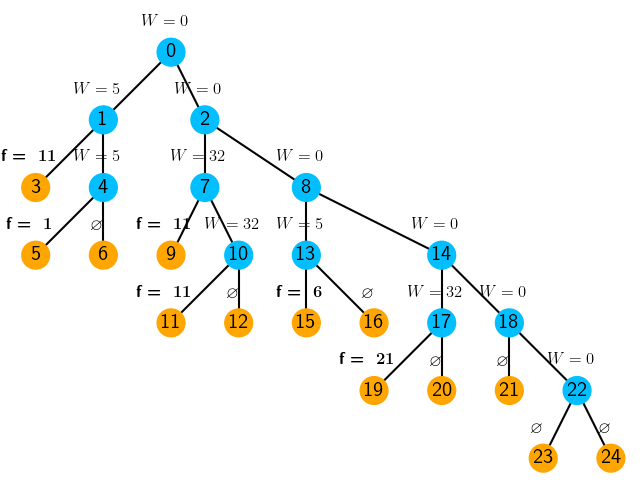
\includegraphics[scale=0.9]{brute_force_tree.png}
  }
  \caption{Решение задачи методом полного перебора}\label{fig:part2_brute_force_tree}
\end{figure}

\paragraph{Решение с помощью МВиГ.}

 На рисунке \cref{fig:part2_branch_and_bound_tree} представлено дерево решения задачи методом ветвей и границ. Теперь закрытие вершины осуществляется в случаях:
 \begin{itemize}
   \item получен новый рекорд размещения;
   \item оценка недопокрытия больше рекорда, полученного на предыдущих итерациях;
   \item нет допустимого размещения БС.
\end{itemize} 


В таблице \cref{tab:branch_and_bound_solution} представлено решение МВиГ. Оптимальное решение получено на 5-ом узле дерева с недопокрытием $f(P)=1$. В ходе движения по дереву поиска, последующие оценки недопокрытия были больше полученного рекорда и данные вершины закрывались. В итоге общее количество узлов составило 16.


\begin{figure}[ht]
  \centerfloat{
      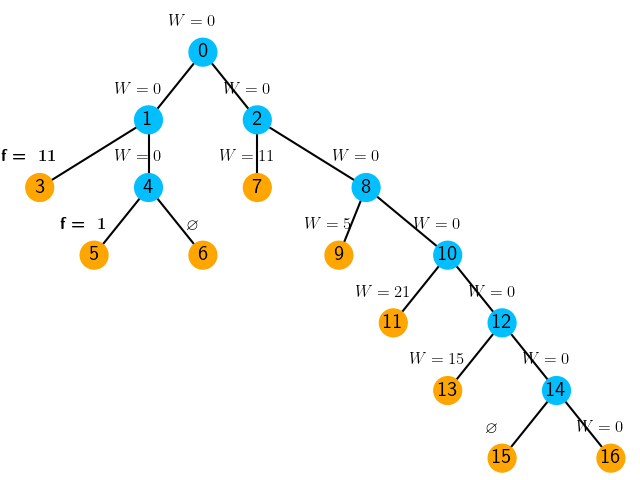
\includegraphics[scale=0.9]{branch_and_bound_tree.png}
  }
  \caption{Решение задачи методом ветвей и границ}\label{fig:part2_branch_and_bound_tree}
\end{figure}

\begin{table}[h!]\centering
  \begin{tabular}{|c|c|c|}\hline
      
      Oценка недопокрытия, $W(G_\nu)$ & Недопокрытие, $f(P)$ & Номер узла дерева, $\nu$\\
      \hline
      11 & Рекорд & 3\\
      \textbf{1} & \textbf{Рекорд} & \textbf{5}\\
      32 &  & 7\\
      5 &  & 9\\
      32 &  & 11\\
      15 &  & 13\\
      \hline

\end{tabular}\caption{Решение полным перебором}\label{tab:branch_and_bound_solution}
\end{table}




% \fixme{===========================}


\section{Сравнения оценок «недопокрытия» для задачи 2, 3 и 4}\label{part4:task_234}

В таблице \cref{tab:part4_estimate_comparison} приведены результаты вычислительного эксперимента, показывающего время решения \underline{\textit{\textbf{задач 2, 3, 4}}} и относительную точность \underline{\textit{\textbf{задачи 3, 4}}} по отношению к \underline{\textit{\textbf{задаче 2}}}.

Для непокрытого участка справа длины $|\beta| = 50$, варьируя количеством неразмещенных БС, а также количеством свободных мест размещения рассчитаем оценку недопокрытия при бюджетном ограничении $C=600$.


Как видно из результатов расчетов в таблице \cref{tab:part4_estimate_comparison}, представляется целесообразным  использовать  \underline{\textit{\textbf{задачу 3}}} в качестве оценки $w_2 (G_\nu )$ для решения задач большой размерности, так как время ее расчета в виде задачи линейного программирования существенно ниже с учетом высокой точности.


% \fontsize{8pt}{8pt}\selectfont
\begin{table}[h!]\centering
  \begin{tabular}{| c  | c  | c | c | c | c | c | c |c | c |}
    
    \hline
    \multirow{2}{*}{\rotatebox{270}{\thead{Количество точек \\ размещения, $m$}}}
    & \multirow{2}{*}{\rotatebox{270}{\thead{Количество  свободных\\ станций,  $|S_\beta|$}}}

    & \multicolumn{2}{|c|}{ЦЛП} 
    & \multicolumn{3}{|c|}{\thead{Задача \\
   <<О ранце>>}} 
    & \multicolumn{3}{|c|}{ЛП} \\\cline{3-10}
 
    &&\rotatebox{270}{Время расчета, сек } 
    &\rotatebox{270}{Недопокрытие, $z$}
    &\rotatebox{270}{Время расчета, сек} 
    &\rotatebox{270}{Недопокрытие, $z$}
    &\rotatebox{270}{Точность, \%}
    &\rotatebox{270}{Время расчета, сек} 
    &\rotatebox{270}{Недопокрытие, $z$}
    &\rotatebox{270}{Точность, \%}\\

    \hline
    5&	6&	0,3250&	436,00&	0,3214&	426,00&	97,71&	0,0047&	436,00&	100,00 \\
    5&	8&	0,3218&	431,00&	0,3582&	398,00&	92,34&	0,0045&	431,00&	100,00 \\
    8&	10&	0,3765&	395,00&	0,3621&	375,00&	94,94&	0,0094&	395,00&	100,00 \\
    8&	12&	0,3746&	390,00&	0,2977&	347,00&	88,97&	0,0094&	390,00&	100,00 \\
    12&	15&	0,3363&	339,00&	0,2960&	309,00&	91,15&	0,0114&	339,00&	100,00 \\
    12&	17&	0,4072&	336,00&	0,3456&	283,00&	84,23&	0,0136&	336,00&	100,00 \\
    18&	20&	0,3558&	265,00&	0,3407&	265,00&	100,00&	0,0121&	265,00&	100,00 \\
    18&	25&	0,3794&	260,00&	0,3096&	259,00&	99,62&  0,0169&	257,60&	99,08 \\
    25&	30&	0,3177&	246,00&	0,3576&	246,00&	100,00&	0,0222&	244,33&	99,32 \\
    25&	45&	0,3539&	229,00&	0,3556&	229,00&	100,00&	0,0494&	226,40&	98,86 \\
    30&	50&	0,2994&	225,00&	0.3146&	225,00&	100,00&	0,0570&	224,13&	99,61 \\
    30&	100& 0,5179& 223,00& 0,5177& 223,00& 100,00& 0,1513& 218,75& 98,09 \\
    \hline
  \end{tabular}\caption{Сравнения оценок «недопокрытия» для задачи ЦЛП и ЛП}\label{tab:part4_estimate_comparison}
  \end{table}
\normalsize


% \fontsize{8pt}{8pt}\selectfont
% \begin{longtable}[c]{| c | c | c | c | c | c | c | c |c | c |}
%     \caption{Сравнения оценок «недопокрытия» для задачи ЦЛП и ЛП}\label{tab:part4_estimate_comparison}\\

%     \hline
%     \multirow{2}{*}{\thead{Количество \\
%         точек \\
%         размещения, \\ $m$}}
%     & \multirow{2}{*}{\thead{Количество \\
%         свободных \\
%         станций, \\ $|S_\beta|$}}

%     & \multicolumn{2}{|c|}{ЦЛП} 
%     & \multicolumn{3}{|c|}{\thead{Задача \\
%     о ранце}} 
%     & \multicolumn{3}{|c|}{ЛП} \\\cline{3-10}
 
%     &&\rotatebox{270}{Время расчета, сек } 
%     &\rotatebox{270}{Недопокрытие, $z$}
%     &\rotatebox{270}{Время расчета, сек} 
%     &\rotatebox{270}{Недопокрытие, $z$}
%     &\rotatebox{270}{Точность, \%}
%     &\rotatebox{270}{Время расчета, сек} 
%     &\rotatebox{270}{Недопокрытие, $z$}
%     &\rotatebox{270}{Точность, \%}\\

%     \hline
%     5&	6&	0,3250&	436,00&	0,3214&	426,00&	97,71&	0,0047&	436,00&	100,00 \\
%     5&	8&	0,3218&	431,00&	0,3582&	398,00&	92,34&	0,0045&	431,00&	100,00 \\
%     8&	10&	0,3765&	395,00&	0,3621&	375,00&	94,94&	0,0094&	395,00&	100,00 \\
%     8&	12&	0,3746&	390,00&	0,2977&	347,00&	88,97&	0,0094&	390,00&	100,00 \\
%     12&	15&	0,3363&	339,00&	0,2960&	309,00&	91,15&	0,0114&	339,00&	100,00 \\
%     12&	17&	0,4072&	336,00&	0,3456&	283,00&	84,23&	0,0136&	336,00&	100,00 \\
%     18&	20&	0,3558&	265,00&	0,3407&	265,00&	100,00&	0,0121&	265,00&	100,00 \\
%     18&	25&	0,3794&	260,00&	0,3096&	259,00&	99,62&  0,0169&	257,60&	99,08 \\
%     25&	30&	0,3177&	246,00&	0,3576&	246,00&	100,00&	0,0222&	244,33&	99,32 \\
%     25&	45&	0,3539&	229,00&	0,3556&	229,00&	100,00&	0,0494&	226,40&	98,86 \\
%     30&	50&	0,2994&	225,00&	0.3146&	225,00&	100,00&	0,0570&	224,13&	99,61 \\
%     30&	100& 0,5179& 223,00& 0,5177& 223,00& 100,00& 0,1513& 218,75& 98,09 \\
%     \hline
% \end{longtable}
% \normalsize








\section{Сравнение модели ЦЛП и комбинаторной модели}

Теперь перейдем к решению задач большей размерности. Для различных случаев числа мест размещения $m$ и числа станций $n$ сравним результаты решения задачи представленными моделями. Оценка сравнения с помощью времени счета необъективна, так как алгоритм МВиГ и комбинаторная модель написаны на интерпретируемом языке Python. Коммерческие продукты представляют быстрые и качественные инструменты. Написание производительного кода для предложенных в данной диссертации моделей является отдельной не простой задачей, выходящей за рамки данного исследования. Коммерческие продукты решающие задачи ЦЛП основаны на алгоритме, предложенный Алисой Лэнд и Элисон Дойг \cite{Land1960}, в котором процедура поиска целочисленного решения также использует МВиГ.  Поэтому для сравнения моделей будет использована характеристика -- число просмотренных вершин в ходе поиска оптимального решения. Для сравнения также будут представлены решения задачи в комбинаторной форме методом полного перебора (МПП).

Для каждого набора станций и мест размещения было рассчитано по 10 примеров с различными параметрами БС. В таблице \cref{tab:models_comparation}приводятся усредненные показатели числа просмотренных вершин дерева поиска по каждым 10 примерам. Результаты решения задачи максимизации покрытия влияют не только от количества точек размещения $n$, но также от их координат. Примем, что для каждой размерности для всех 10 примеров координаты фиксированные для всех моделей: МПП, МВиГ и ЦЛП. 


\begin{table}
  \caption{Результаты численного решения.}\label{tab:models_comparation}
  \begin{tabular}{|ccc|*{3}{c}|} \cline{3-6}
  \hline
  \textbf{Число точек} & \textbf{Число} &\textbf{Количество} & \multicolumn{3}{c|}{\textbf{Количество пройденных}}\\ 
  \textbf{размещения,} & \textbf{cтанций,} & \textbf{вариантов} & \multicolumn{3}{c|}{\textbf{узлов дерева поиска, $\nu$}}\\
  \cline{4-6}
  \textbf{$n$} & \textbf{$m$} &\textbf{размещения, $\gamma$} & \textbf{МПП}& \textbf{МВиГ} & \textbf{ЦЛП} \\ 
  \hline
  7 &  4 & 840 & 3122 & 360 &  \textbf{275} \\
  7 &  5 & 2 520 & 16 114 & 560  &  \textbf{45}  \\
  7 &  6 & 5 040 & 59 564 & 364  &  \textbf{19}  \\
  8 &  4 & 1 680 &  4954 &  434 &   \textbf{189} \\
  8 &  5 & 6 720 & 6720 & \textbf{852}  &  878 \\
  8 &  6 & 20 160 &  15 9170 & 592  & \textbf{185}  \\
  9  &  4 & 3 024 & 9 882 & \textbf{458} & 5511 \\
  9  &  5 & 15 120&  58 190 &  \textbf{768} &  1236\\
  9  &  6 & 60 480&  366 512 &  \textbf{720} & 13294 \\
  10 &  4 & 5 040&  14 868&  \textbf{800}&  6243\\
  10 &	5 & 30 240&  113 932&  \textbf{414}&  8043\\
  10 &	6 & 151 200&  828 952&  \textbf{40 872}&  71587\\
  11 &  4 & 7 920& 23 482&  \textbf{354} & 15538\\
  11 &	5 & 55 440& 204 894& \textbf{9 138}&  74440\\
  11 &	6 & 332 640& 1 592 500 & \textbf{88 002} & 413 767 \\
  \hline
  \end{tabular}
\end{table} 

Жирным цветом в колонках пройденных узлов в ходе движения по дереву поиска МПП, МВиГ и ЦЛП выделены минимальные значения для фиксированных значений $n$ и $m$ (размерностей задачи). Как видно из результатов сравнения, при увеличении размерности задачи разработанный алгоритм метода ветвей и границ для комбинаторной модели показывает лучшие результаты по сравнению с математической моделью ЦЛП.